\section*{Problem 8.1\footnote[1]{Problem 8 kommt 2mal vor, sind aber unterschiedliche Aufgaben} - SISO Rayleigh fading channel}
\begin{align*}
	&\overline{\mathrm{SER}}=\mathbb{E}_{\left|h\right|^{2}}\left\{\mathrm{SER}\left(\left|h\right|^2\right)\right\}& \\
	& 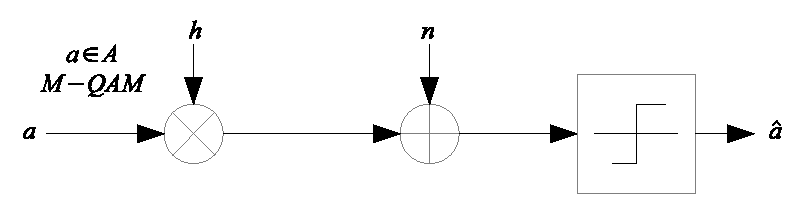
\includegraphics[width=0.6\textwidth]{rx_chain.eps} & \\
	&\mathrm{SER}\left(\left|h\right|^2\right)=C_{\mathcal{A}}\mathrm{Q}\left(\sqrt{d_\mathrm{min}^2\frac{E_{b}}{N_0}}\left|h\right|^2\right)& \\
	&\qquad C_{\mathcal{A}}=3\quad\left(\text{16-QAM}\right)\qquad\qquad C_{\mathcal{A}}=2\quad\left(\text{4-QAM}\right)& \\
	&\qquad =C_{\mathcal{A}}\mathrm{Q}\left(\sqrt{\underbrace{\frac{d_\mathrm{min}^2}{\ld(\left(M\right)}}_{d_{\mathcal{A}^2}} \underbrace{\frac{E_{s}}{N_0}}_{\gamma}\left|h\right|^2}\right)=C_{\mathcal{A}}\mathrm{Q}\left(\sqrt{d_\mathcal{A}^2\gamma\left|h\right|^2}\right)& \\
	&h\sim CN\left(0,1\right)\quad\rightarrow\quad\left|h\right|^2\text{ is exponentially distributed with variance 1}& \\
	&\quad\rightarrow\overline{\mathrm{SER}}=\int\limits_0^\infty \underbrace{f_{\left|h\right|^2}\left(x\right)}_{\text{pdf of }\left|h\right|^2} \mathrm{SER}\left(x\right)\mathrm{d}x=\int\limits_0^\infty\mathrm{e}^{-x}C_{\mathcal{A}}\mathrm{Q}\left(\sqrt{d_\mathcal{A}^2\gamma\left|h\right|^2}\right)\mathrm{d}x& \\
	&\qquad\mathrm{Q}\left(x\right)=\frac{1}{2\pi}\int\limits_x^\infty e^{-\frac{t^2}{2}}\mathrm{d}t& \\
	&\quad\rightarrow\quad\overline{\mathrm{SER}}=\int\limits_0^\infty e^{-x}C_\mathcal{A}\frac{1}{\sqrt{2\pi}}\int\limits_{\sqrt{d_\mathcal{A}^2\gamma_x}}^\infty e^{-\frac{t^2}{2}}\mathrm{d}t\,\mathrm{d}x& \\
	&\quad\rightarrow\quad\text{change the order of integrals}& \\
	&\quad\rightarrow\quad\overline{\mathrm{SER}}=\frac{C_\mathcal{A}}{\sqrt{2\pi}}\int\limits_{\sqrt{d_\mathcal{A}^2\gamma_x}}^\infty\int\limits_0^\infty e^{-x}e^{-\frac{t^2}{2}}\mathrm{d}x\,\mathrm{d}t&
\end{align*}
\begin{align*}
	& 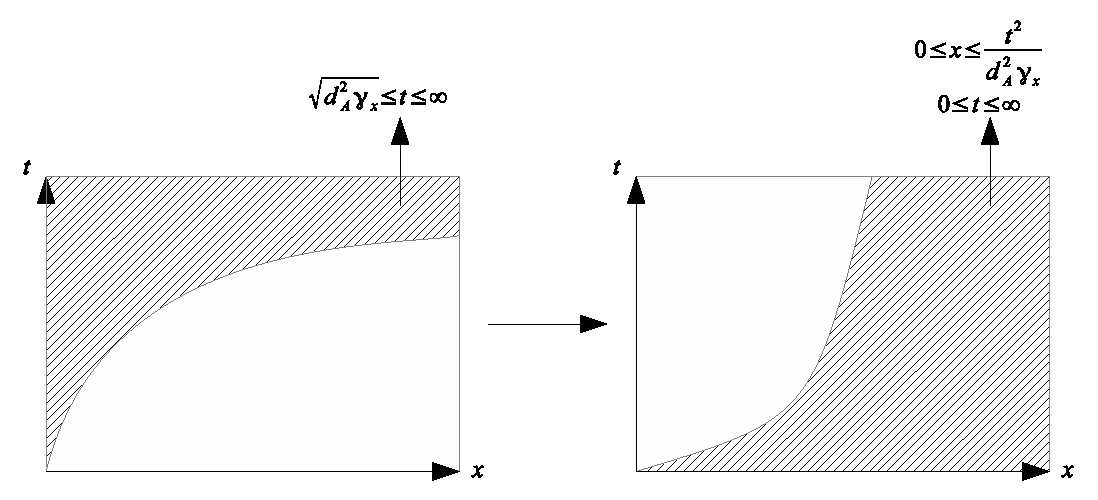
\includegraphics[width=1\textwidth]{integration.eps} & \\
	\overline{\mathrm{SER}} & =\frac{C_\mathcal{A}}{\sqrt{2\pi}}\int\limits_0^\infty\int\limits_0^\frac{t^2}{d_\mathcal{A}^2\gamma}e^{-x}e^{-\frac{t^2}{2}}\mathrm{d}x\,\mathrm{d}t=\frac{C_\mathcal{A}}{\sqrt{2\pi}}\int\limits_0^\infty e^{-\frac{t^2}{2}}\left[e^{-x}\right]_0^{\frac{t^2}{d_\mathcal{A}^2\gamma}}\mathrm{d}t= \\
	& =\frac{C_\mathcal{A}}{\sqrt{2\pi}}\int\limits_0^\infty e^{-\frac{t^2}{2}}\left(-e^{-\frac{t^2}{d_\mathcal{A}^2\gamma}}+1\right)\mathrm{d}t= \\
	& =\frac{C_\mathcal{A}}{\sqrt{2\pi}}\int\limits_0^\infty\left(e^{-\frac{t^2}{2}}-e^{-\frac{t^2}{2}\left(1+\frac{2}{d_\mathcal{A}^2\gamma}\right)}\right)\mathrm{d}t= \\
	& =\frac{C_\mathcal{A}}{\sqrt{2\pi}}\left(\sqrt{2\pi}\underbrace{\mathrm{Q}\left(0\right)}_{\frac{1}{2}}-\sqrt{\frac{2\pi}{1+\frac{2}{d_\mathcal{A}^2\gamma}}}\underbrace{\mathrm{Q}\left(\sqrt{1+\frac{2}{d_\mathcal{A}^2\gamma}}0\right)}_{0}\right)= \\
	& =\frac{C_\mathcal{A}}{2}\left(1-\sqrt{\frac{1}{1+\frac{2}{d_\mathcal{A}^2\gamma}}}\right)=\boxed{\frac{C_\mathcal{A}}{2}\left(1-\sqrt{\frac{d_\mathcal{A}^2\gamma}{d_\mathcal{A}^2\gamma+2}}\right)} \\
\end{align*}

\subsection*{d)}
\begin{align*}
	& \text{Asymptotic $\overline{\mathrm{SER}}$ if $\gamma\rightarrow\infty$} \\
	& \overline{\mathrm{SER}}=\frac{C_\mathcal{A}}{2}\left(1-\sqrt{\frac{d_\mathcal{A}^2\gamma}{d_\mathcal{A}^2\gamma+2}}\right) \\
	& \qquad C_\mathcal{A}:\text{ average number of nearest neighbours in the constellation diagram} \\
	& \text{Taylor series:}\quad f\left(x\right)\approx f\left(x_0\right)+\left(x-x_0\right)f'\left(x_0\right)+\frac{\left(x-x_0\right)^2}{2}f''\left(x_0\right)+\ldots \\
	& \text{uppper bound:}\quad f\left(x\right)\approx f\left(x_0\right)+\left(x-x_0\right)f'\left(x_0\right) \\
	& \quad x_0=0\quad\rightarrow\quad f\left(x\right)=f\left(0\right)+xf'\left(0\right) \\
	& \quad x=\frac{1}{d_\mathcal{A}^2\gamma}\text{ if }\gamma\rightarrow\infty\quad\Rightarrow\quad x=0 \\
	& \overline{\mathrm{SER}}\left(x\right)=\frac{C_\mathcal{A}}{2}\left(1-\sqrt{\frac{1}{1+2x}}\right) \\
	& \overline{\mathrm{SER}}\left(x\right)\le\overline{\mathrm{SER}}\left(0\right)+x\mathrm{SER}'\left(0\right) \\
	& \quad\overline{\mathrm{SER}}\left(0\right)=\frac{C_\mathcal{A}}{2}\left(1-\sqrt{\frac{1}{1}}\right)=0 \\
	& \quad\overline{\mathrm{SER}'}\left(x\right)=-\frac{C_\mathcal{A}}{2}\frac{1}{2\sqrt{\frac{1}{1+2x}}}\frac{-1}{\left(1+2x\right)^2}2\quad\Rightarrow\quad\overline{\mathrm{SER}'}\left(0\right)=-\frac{C_\mathcal{A}}{2} \\
	& \quad\rightarrow\quad\overline{\mathrm{SER}}\left(x\right)\le\frac{C_\mathcal{A}}{2}x\quad\rightarrow\quad\boxed{\overline{\mathrm{SER}}\left(\gamma\right)\le\frac{C_\mathcal{A}}{2}\frac{1}{d_\mathcal{A}^2\gamma}} \\
	& \mathrm{SER}\left(\left|h\right|^2\right)=C_\mathcal{A}\mathrm{Q}\left(\sqrt{d_\mathcal{A}^2\gamma\|h\|^2}\right) \\
	& \qquad\text{we could have used Chernoff bound: }\mathrm{Q}\left(x\right)\le\frac{1}{2}\mathrm{e}^{-\frac{x^2}{2}} \\
	& \mathrm{SER}\left(\left|h\right|^2\right)\le\frac{C_\mathcal{A}}{2}e^{-\frac{d_\mathcal{A}^2\|h\|^2\gamma}{2}}\quad\rightarrow\quad\ldots\quad\rightarrow\quad\boxed{\overline{\mathrm{SER}}\le C_\mathcal{A}\frac{1}{d_\mathcal{A}^2\gamma}} \\
\end{align*}